% Measuring Before Believing — technical report (draft, Phase 4)
% Every number in this file is mapped to a row of claims.csv (IDs in %-comments: [Cnn]).
% Figure captions are generated (figures/captions.tex); the appendix hash table is generated
% (appendix_hashes.tex). Build: tectonic main.tex
\documentclass[11pt,a4paper]{article}
\usepackage[margin=2.4cm]{geometry}
\usepackage{fontspec}
\usepackage{amsmath}
\usepackage{graphicx}
\usepackage{booktabs}
\usepackage{longtable}
\usepackage{array}
\usepackage{xcolor}
\usepackage{etoolbox}
\usepackage[font=small,labelfont=bf,justification=raggedright,singlelinecheck=false]{caption}
\usepackage[numbers,sort&compress]{natbib}
\usepackage[hidelinks]{hyperref}
\usepackage{enumitem}
\usepackage{placeins}
\setlist{itemsep=2pt,topsep=4pt}
\setlength{\parskip}{3pt}
\renewcommand{\arraystretch}{1.12}
\newcommand{\R}{\ensuremath{R}}
% generated by paper/tools/captions_to_tex.py from figures/captions.md -- do not edit
\csdef{cap-F1}{Harness calibration on identical data (165,437 M5 bars) and identical strategy code; the two runs differ only in the window-slicing rule. (a) The hatched bar is the legacy per-leg statistic; moving to the per-signal unit and then to close-time slicing reduces t from +3.345 to +2.453 to +0.917. (b) Per-signal expectancy with a 95\% interval recovered from the reported t (SE = mean/t). Limit-fill configuration, costs on. \emph{Source:} \texttt{report\_calib\_v1\_full.json} (SHA-256 \texttt{611cf0bbc7003970}\ldots{}); \texttt{report\_calib\_v2\_full.json} (SHA-256 \texttt{c71ed4c181c1f610}\ldots{}).}
\csdef{cap-F2}{Cumulative return (top) and drawdown from running peak (bottom) for the two calibration runs in Figure~\ref{fig:F1}, as percentages of the simulated starting balance, sampled at each day's last bar. Daily sampling understates the intrabar maximum drawdown reported by the backtester (legacy 4.82\%, harness-v2 5.43\%). Return falls under the corrected harness while maximum drawdown does not. \emph{Source:} \texttt{report\_calib\_v1\_full.json} (SHA-256 \texttt{611cf0bbc7003970}\ldots{}); \texttt{report\_calib\_v2\_full.json} (SHA-256 \texttt{c71ed4c181c1f610}\ldots{}).}
\csdef{cap-F3}{Share of 1000 random M5 decision steps at which the H1 window contained a bar that had not yet closed. Legacy slicing: 915/1000; theoretical rate for M5 steps within an hour: 55/60; harness-v2: 0/1000 (mandatory test, fixed seed, re-run 2026-11-01). \emph{Source:} \texttt{paper/\allowbreak{}figures/\allowbreak{}data/\allowbreak{}test\_no\_lookahead\_run\_2026-11-01.txt} (SHA-256 \texttt{8665c4f57915bc68}\ldots{}); \texttt{tests/\allowbreak{}test\_no\_lookahead.py} (SHA-256 \texttt{875305ae0c521f07}\ldots{}).}
\csdef{cap-F4}{Pre-registered supply/demand-zone strategy on the DEV partition (2024). T1 is the frozen specification; T2--T4 vary the two zone-quality parameters (all four runs are rows 1--4 of the append-only trial ledger). Points are per-signal expectancy net of costs; bars are 95\% intervals recovered from the reported t (SE = mean/t). The dashed line is the pre-registered gate. T1 t = $-$2.793. Every point estimate is negative and every interval lies below the gate. \emph{Source:} \texttt{report\_zone\_dev\_t1.json} (SHA-256 \texttt{8e78f735b0f4b135}\ldots{}); \texttt{report\_zone\_dev\_t2.json} (SHA-256 \texttt{680cfa7bc39d4ac3}\ldots{}); \texttt{report\_zone\_dev\_t3.json} (SHA-256 \texttt{cabb08e7febc8bc5}\ldots{}); \texttt{report\_zone\_dev\_t4.json} (SHA-256 \texttt{3b6de201b05e0ac0}\ldots{}); \texttt{trials.csv} (SHA-256 \texttt{8334fec3d4328530}\ldots{}); \texttt{specs/\allowbreak{}phase1\_zone\_spec\_v1.md} (SHA-256 \texttt{03ddb7b216a925c0}\ldots{}).}
\csdef{cap-F5}{Signal funnel for the frozen zone specification on DEV. Touches not traded: 74 skipped by the one-position limit and 28 by the gap-through-stop rule. \emph{Source:} \texttt{report\_zone\_dev\_t1.json} (SHA-256 \texttt{8e78f735b0f4b135}\ldots{}).}
\csdef{cap-F6}{The 15 documented ideas and their epistemic labels (Table~\ref{tab:ideas}). Tiles marked † (dashed border) rest on a dated contemporaneous record whose generating script was not re-run (Tier B). \textsuperscript{1}Premium present but tail risk incompatible with a 10\% drawdown cap. \textsuperscript{2}Phase-1 gate passed; no significant alpha beyond a buyable managed-futures ETF. 'Not supported' means no evidence of edge, not evidence of no edge. Per-idea sources are listed by claim ID in the claims table. \emph{Source:} \texttt{paper/\allowbreak{}claims.csv} (SHA-256 \texttt{3deb8b61a7ee262f}\ldots{}).}
\csdef{cap-F7}{Why the re-measurement is weak evidence. Per-signal t for the $\geq$2-timing-flag SMC subset: in-sample (subset chosen after seeing these data) t = +3.045, n = 228; re-run windows t = +0.06, n = 37. The re-run windows lie inside the in-sample period and are not an out-of-sample test. The band shows the t expected at each n if the in-sample per-signal Sharpe (0.202) were true; the re-measurement falls inside it. Both sides ran on the legacy harness. \emph{Source:} \texttt{report\_full.json} (SHA-256 \texttt{a7fedee66dc7badc}\ldots{}); \texttt{report\_w1.json} (SHA-256 \texttt{8c76ed83a99772f3}\ldots{}); \texttt{report\_w2.json} (SHA-256 \texttt{476833c1c1aa009c}\ldots{}); \texttt{report\_w3.json} (SHA-256 \texttt{cd33449fc8eec236}\ldots{}); \texttt{report\_w4.json} (SHA-256 \texttt{a849526720e1a6c8}\ldots{}); \texttt{report\_w5.json} (SHA-256 \texttt{ecfc8198f9d91cf1}\ldots{}).}
\csdef{cap-F8}{Runtime architecture, drawn from the publish/subscribe calls in the code (event-bus topic names in monospace). Both halt paths (reconciliation desync in the trade logger; unconfirmed fill in the order executor) raise SYSTEM\_SHUTDOWN, which stops trading without closing positions. The decision path from bars to orders is deterministic; the optional language-model component is an hourly higher-timeframe advisory that is disabled by default. Secondary components (break-even monitor, pending-order manager, notifier, status exporter, system monitor, emergency liquidator) are omitted for legibility. \emph{Source:} \texttt{main.py} (SHA-256 \texttt{a01eb656a6ec7efd}\ldots{}); \texttt{core/\allowbreak{}event\_bus.py} (SHA-256 \texttt{9d08645d45403b69}\ldots{}); \texttt{agents/\allowbreak{}risk\_manager.py} (SHA-256 \texttt{1dfa09df59084abe}\ldots{}); \texttt{execution/\allowbreak{}order\_executor.py} (SHA-256 \texttt{f3fdfe9f9b680891}\ldots{}); \texttt{memory/\allowbreak{}trade\_logger.py} (SHA-256 \texttt{1688bb607d715397}\ldots{}).}
\csdef{cap-F9}{Order of events in the zone study, from git commit timestamps and the trial ledger's own timestamps (UTC; gaps between consecutive events on the left). The specification (prior, gate G2, partitions) was committed 21.4 h before the first ledger row was written. Ledger timestamps record when a run completed; start times were not recorded, so the first run may have begun shortly before the engine commit. The spec's own provenance appendix states that no statistic was computed on any partition before the freeze. The only later spec change was that provenance appendix (40 lines added, 0 deleted). Rows 2--4 were chosen after row 1 under the spec's DEV-tuning allowance. Commit times are self-reported by the author's machine and are not externally notarised. \emph{Source:} \texttt{paper/\allowbreak{}figures/\allowbreak{}data/\allowbreak{}git\_timeline\_utc.txt} (SHA-256 \texttt{94bca4ed34c7db10}\ldots{}); \texttt{trials.csv} (SHA-256 \texttt{8334fec3d4328530}\ldots{}); \texttt{specs/\allowbreak{}phase1\_zone\_spec\_v1.md} (SHA-256 \texttt{03ddb7b216a925c0}\ldots{}); \texttt{paper/\allowbreak{}figures/\allowbreak{}data/\allowbreak{}spec\_appendix\_numstat\_8634f34.txt} (SHA-256 \texttt{4f2bfe6ee91d7c32}\ldots{}).}


\title{Measuring Before Believing:\\[2pt]
\large A Pre-Registered Falsification Study of Retail Price-Structure Strategies on XAUUSD}
\author{SuperKICKY01\\\small Independent student researcher, Thailand\\\small Independent technical report --- not peer-reviewed}
\date{November 2026}

\begin{document}
\maketitle

\begin{abstract}
\noindent
Retail trading education promotes entry rules based on visible price structure, such as order
blocks and supply/demand zones. This report asks whether two such rule families show measurable
per-signal edge on 5-minute XAUUSD data once the backtest is causal and inference uses the
independent unit. Two defects were found in the project's own legacy backtester:
higher-timeframe windows contained a still-forming bar at 91.5\% of decision steps, and
significance was computed per position leg rather than per signal. Correcting both on identical
data and code reduced the order-block strategy's per-signal $t$-statistic from $+2.45$ to $+0.92$
($n=77$). A supply/demand-zone strategy was then specified and committed before its first backtest result
and run on a development partition only: per-signal expectancy $-0.143\R$, $t=-2.79$ ($n=406$),
against a pre-registered requirement of at least $+0.15\R$; three further runs selected after the
first also had negative expectancy. The evaluation partitions were left unused. Fifteen
documented ideas are reported with explicit evidence labels, and three errors in earlier project
documents are corrected. The contribution is a documented case study and open validation
tooling, not a new method.
\end{abstract}

% ════════════════════════════════════════════════════════════════════════════
\section{Introduction}

Strategies built on ``price structure''---order blocks, breaks of structure, supply and demand
zones---are widely taught to retail traders. Their premise is that price revisits levels at
which orders are concentrated, and that a trader who enters on the revisit is paid for doing so.
The evidence on retail speculative trading is not encouraging: individual investors in aggregate
lose from trading \citep{barber2009lose}, and among day traders only a small minority show
persistent ability to profit \citep{barber2014daytrading}. Whether a specific retail rule has an
edge is, however, an empirical question that a careful backtest can address cheaply.

This report documents one attempt to answer that question for XAUUSD (spot gold against the US
dollar) on 5-minute bars, and in particular what was needed before the answer could be trusted.
The research question is:

\begin{quote}
\emph{Do two retail price-structure rule families---an order-block confluence rule and a
supply/demand-zone rule---show measurable per-signal edge on XAUUSD M5 data when the backtest is
causal and inference is performed on the independent unit?}
\end{quote}

The contributions are modest and are stated as such:
\begin{enumerate}
\item A worked case of how two defects in a backtest harness inflated an apparent edge,
quantified on identical data and identical strategy code (Section~\ref{sec:res-g0}).
\item A pre-registered falsification of a supply/demand-zone strategy with an append-only trial
ledger, stopped at the development stage so that the evaluation data remain unused
(Section~\ref{sec:res-zone}).
\item A register of fifteen documented ideas with explicit evidence labels and evidence tiers,
including ideas that were not tested (Section~\ref{sec:res-register}).
\item The validation tooling itself: close-time window slicing with a mandatory test,
per-signal statistics, and the trial ledger, published with hashes of every evidence file
(Appendix~\ref{app:repro}).
\end{enumerate}
No new statistical method is proposed, and no claim is made that price structure cannot carry
information in general. ``No evidence of edge'' is not the same statement as ``no edge''.

% ════════════════════════════════════════════════════════════════════════════
\section{Related work}

\paragraph{Backtest overfitting and selection.}
When many configurations are tried and the best is reported, its Sharpe ratio is biased upward.
The Deflated Sharpe Ratio corrects a reported Sharpe ratio for the number of trials and for
non-normal returns \citep{bailey2014dsr}. \citet{bailey2014pseudo} argue that backtest
overfitting is a plausible reason that strategies which look profitable in backtests fail out of
sample, and \citet{bailey2017pbo} propose combinatorially symmetric cross-validation to estimate
the probability that a selected configuration is overfit. Purged cross-validation for financial
time series is described by \citet{lopezdeprado2018afml}.

\paragraph{Multiple testing in finance.}
\citet{harvey2016cross} treat the literature's many claimed return predictors as a multiple-testing
problem and argue that a new factor should clear a $t$-statistic of about 3.0 rather than 2.0.
False-discovery-rate control \citep{benjamini1995fdr} is the standard alternative to
family-wise error control when many hypotheses are screened; it is used in one of the ideas in
Section~\ref{sec:res-register}.

\paragraph{Retail trader performance.}
Using complete trading records from Taiwan, \citet{barber2009lose} find that individual investors'
trades produce large systematic losses, and \citet{barber2014daytrading} find that although a
small group of day traders predictably earns positive returns, the cross-section is dominated by
losses.

\paragraph{Order clustering at price levels.}
The closest institutional evidence for why price levels might matter comes from foreign-exchange
order data. \citet{osler2003currency} documents that take-profit orders cluster at round numbers
and stop-loss orders cluster just beyond them, and uses this to explain why trends tend to reverse
at, or accelerate through, such levels. \citet{osler2005stoploss} finds that rapid price moves are
associated with the execution of clustered stop-loss orders. These findings concern levels at
which orders are documented to sit; whether the levels that retail rules draw coincide with such
clusters is a separate question, and the per-touch payoff test in Section~\ref{sec:res-zone}
measures the consequence directly.

\paragraph{Pre-registration.}
Fixing hypotheses and analysis plans before seeing outcomes separates prediction from
postdiction \citep{nosek2018prereg}. The zone study in Section~\ref{sec:method-prereg} follows
this practice.

\paragraph{Other strategy classes.}
Time-series momentum \citep{moskowitz2012tsmom} and standard errors that are robust to
heteroskedasticity and autocorrelation \citep{newey1987hac} appear in two of the registered
ideas.

% ════════════════════════════════════════════════════════════════════════════
\section{System}
\label{sec:system}

The studies run on the backtesting side of a live trading system written in asynchronous Python
for the MetaTrader~5 (MT5) platform. The live system is described briefly because its design
determines what the backtest has to imitate (Figure~\ref{fig:F8}).

\paragraph{Architecture.}
Components communicate through an in-process publish/subscribe event bus; \texttt{main.py}
starts thirteen core tasks and one optional task. % [C71]
All blocking calls to the MT5 terminal run in worker threads. The path from incoming bars to an
order is deterministic. A language-model component was removed from that path on 2026-06-05 and
survives only as an optional hourly higher-timeframe advisory, disabled by default. % [C62]

\paragraph{Risk engine.}
Every candidate trade passes nine numbered deterministic vetoes and a pre-emptive daily-drawdown
circuit breaker: a news blackout, daily drawdown, total drawdown, concurrent position slots,
duplicate direction, stop-loss too wide relative to the average true range (ATR), stop-loss too
tight relative to ATR, zero lot size, and a margin pre-flight check. % [C57]

\paragraph{Execution safety.}
A broker acknowledgement is not treated as a fill: the order executor waits until the
corresponding entry deal appears in the broker's deal history before publishing the trade as
executed, and halts the system if confirmation does not arrive. % [C58, C72]
A periodic reconciliation compares open broker positions with the trade database and halts on a
mismatch. % [C59]
A halt stops new trading but deliberately does not close positions; their broker-side stop-loss
and take-profit orders remain in force. % [C60]
A fault-injection run with a hard process kill and recovery check passed, with no position ever
recorded for an unfilled order. % [C61]

\begin{figure}[htbp]
\centering
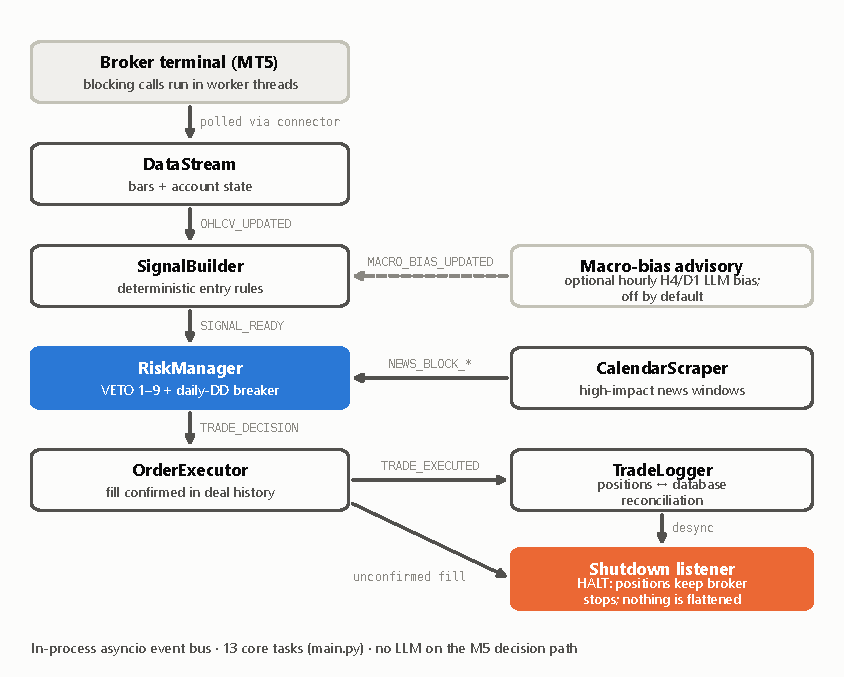
\includegraphics[width=0.82\linewidth]{figures/F8_architecture.pdf}
\caption{\csuse{cap-F8}}
\label{fig:F8}
\end{figure}

% ════════════════════════════════════════════════════════════════════════════
\section{Methodology}
\label{sec:method}

\subsection{Data}
All backtests use Dukascopy BID quotes, resampled from 1-minute to 5-minute bars: 165,437 bars
from 2024-01-01 to 2026-05-06. % [C14, C63]
The price file is not redistributed (Appendix~\ref{app:repro}); its SHA-256 hash and the fetch
script are published so that the file can be regenerated and checked.

\subsection{Close-time window slicing (harness-v2)}
\label{sec:method-slicing}
A decision on the 5-minute (M5) bar that closes at time $T$ may use only higher-timeframe bars
that had \emph{closed} by $T$. The legacy harness selected bars by their open-time label
($\text{label}\le T$), which admits the hourly (H1) bar that opened before $T$ but has not yet
closed. For M5 decisions inside an hour this happens at 11 of every 12 steps; the bar's full
high, low and close then leak up to 55 minutes of future prices into the decision. The corrected
harness keeps a bar only if its open time plus its duration is at most $T$. A mandatory test
draws 1,000 random replay steps and asserts that no window contains a bar closing after the
decision time; it passes 1,000/1,000, and on the same steps the legacy rule would have included a
forming H1 bar 915 times (Figure~\ref{fig:F3}). % [C01–C04]

\begin{figure}[htbp]
\centering
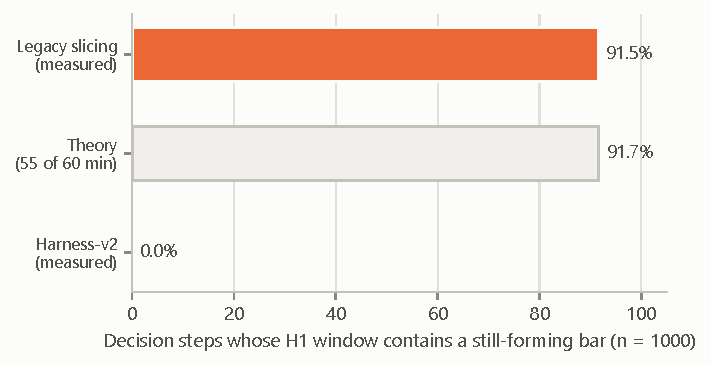
\includegraphics[width=0.66\linewidth]{figures/F3_forming_bar.pdf}
\caption{\csuse{cap-F3}}
\label{fig:F3}
\end{figure}

\subsection{Per-signal statistics}
\label{sec:method-persignal}
Each signal opens two positions (legs) with different take-profit levels and the same entry and
stop. The legs' outcomes are strongly correlated, so treating them as independent overstates
significance by up to a factor of $\sqrt{2}$. The canonical unit is therefore the signal. Each
signal's net profit and its net result in units of $\R$---the amount risked on the signal,
computed with the same denominator used for lot sizing---are aggregated over its legs, and
$t = \bar{x}/(s/\sqrt{n})$ with sample standard deviation $s$ ($n-1$ degrees of freedom). % [C16]
Per-leg statistics appear in this report only where a legacy number is quoted, and are labelled.

\subsection{Pre-registration of the zone study}
\label{sec:method-prereg}
\begin{figure}[tbp]
\centering
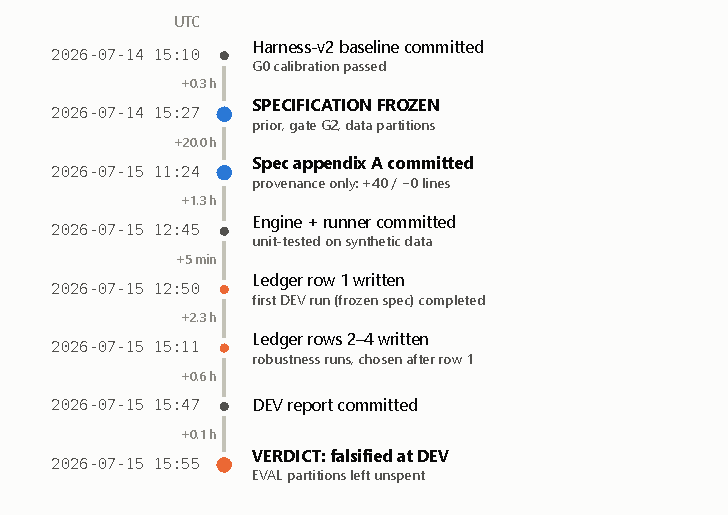
\includegraphics[width=0.54\linewidth]{figures/F9_preregistration_timeline.pdf}
\caption{\csuse{cap-F9}}
\label{fig:F9}
\end{figure}
A specification of the supply/demand-zone strategy was committed to version control, together
with a prior, a pass/fail gate and data partitions, 21.4 hours before the first backtest result
was recorded (Figure~\ref{fig:F9}). % [C68, C70]
\begin{itemize}
\item \textbf{Prior:} probability of a durable edge about 3--5\%, because the strategy belongs to
the same family as the order-block rule already found wanting. % [C18]
\item \textbf{Rules:} zones are built on closed H1 bars from two-bar fractal swings followed by
an impulse of at least $1.5\times$ATR(14) within three bars; only the first touch of a zone
within 72 H1 bars is traded; entry is a market order at the next M5 open with 0.25 adverse
slippage; the stop is at the zone's far edge $\pm\,0.2\times$ATR; two legs target $1\R$ and
$2\R$, with the second moved to break-even after the first fills; risk is 0.5\% per signal and
transaction costs are charged. % [C21 params; spec L49–150]
\item \textbf{Partitions:} DEV = 2024 (tuning allowed, every run logged); EVAL-1 = 2025 H1;
EVAL-2 = 2025 H2; EVAL-3 = 2026 January--June; FRESH = data after 2026-06-30. % [C20]
\item \textbf{Gate G2} (all required): per-signal $t\ge2.5$ in at least two of three EVAL
windows and pooled; expectancy at least $+0.15\R$ after costs; Deflated Sharpe Ratio above 0.95
at $N$ equal to the number of ledger rows; maximum drawdown at most 6\% at 0.5\% risk. % [C19]
\end{itemize}
The only change to the specification after it was frozen was an appendix documenting parameter
provenance, which added 40 lines and deleted none. % [C69]

\subsection{Append-only trial ledger}
Every run that touches price data is appended to a ledger with its parameters and results; rows
are never deleted, and the row count is the $N$ used to deflate Sharpe ratios. Ledger timestamps
are written when a run completes; start times are not recorded. % [C29, C70]

\subsection{Controls}
A positive control---a synthetic series with a planted signal---was used for one of the
registered ideas (idea~8 in Table~\ref{tab:ideas}). A null control on the corrected harness, in
which entries are randomised and the expected result is zero, has not yet been run; this is
listed as a limitation (Section~\ref{sec:limits}).

% ════════════════════════════════════════════════════════════════════════════
\FloatBarrier
\section{Results}
\label{sec:results}

\subsection{Order-block strategy: the corrected-harness calibration}
\label{sec:res-g0}

The legacy order-block confluence strategy, labelled SMC (``smart money concepts'') in the
figures (configuration frozen in May 2026: minimum score 75,
0.65\% risk, transaction costs on, limit-order fills) was re-run twice on identical data and
identical current code. % [C06]
The two runs differ only in the window-slicing rule: V1 uses the legacy rule and V2 the
close-time rule. Table~\ref{tab:g0} and Figure~\ref{fig:F1} report the result.

\begin{table}[htbp]
\centering\small
\caption{Calibration of the harness on identical data and code. Per-signal rows are canonical;
per-leg rows are the legacy statistic, shown for comparison. The recorded column is the
artifact from May 2026, produced by earlier code.}
\label{tab:g0}
\begin{tabular}{@{}lrrr@{}}
\toprule
 & Recorded (legacy) & V1 legacy slicing & V2 close-time slicing \\
\midrule
Per-leg profit factor / $t$ & 1.402 / $+3.161$ & 1.490 / $+3.345$ & 1.220 / $+1.250$ \\ % [C05, C09, C10]
Signals ($n$) & --- & 89 & 77 \\ % [C07, C08]
Per-signal profit factor & --- & 1.748 & 1.258 \\
Per-signal expectancy ($\R$) & --- & $+0.346$ & $+0.133$ \\
Per-signal $t$ (profit / $\R$) & --- & $+2.453$ / $+2.531$ & $+0.917$ / $+0.928$ \\
Return over 28.2 months (\%) & $+21.19$ & $+21.69$ & $+6.67$ \\
Maximum drawdown (\%) & 5.44 & 4.82 & 5.43 \\
\bottomrule
\end{tabular}
\end{table}

\begin{figure}[htbp]
\centering
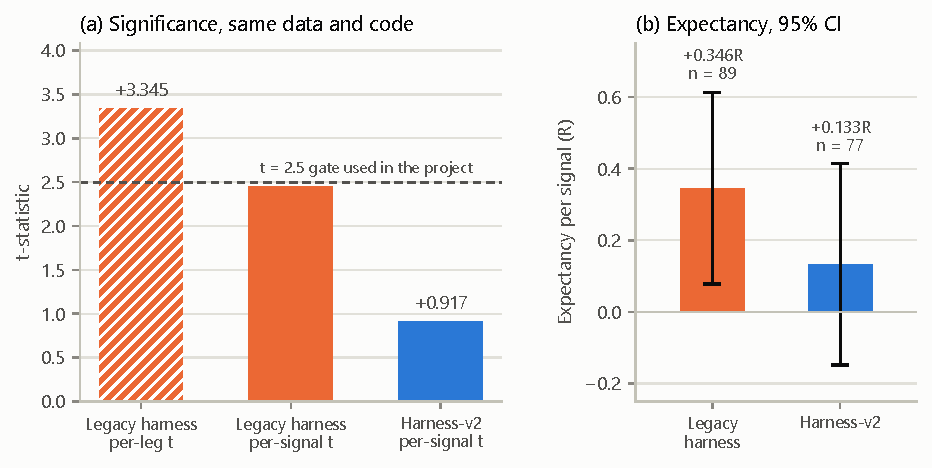
\includegraphics[width=\linewidth]{figures/F1_g0_calibration.pdf}
\caption{\csuse{cap-F1}}
\label{fig:F1}
\end{figure}

Removing the lookahead alone (V1 to V2) reduced the per-signal $t$-statistic from $+2.453$ to
$+0.917$ and per-signal expectancy by 62\%, and removed 69\% of net profit. % [C07, C08, C12, C13]
On the legacy run, counting legs instead of signals inflated $t$ by a further factor of 1.36
(3.345 versus 2.453). % [C11]
The maximum drawdown did not fall with the expectancy (Figure~\ref{fig:F2}). Under the corrected
harness the evidence for an edge is $n=77$ signals with $t=+0.92$, which is below every gate used
in the project, and the 95\% interval for expectancy includes zero. This is the primary evidence on
the order-block strategy.

\begin{figure}[htbp]
\centering
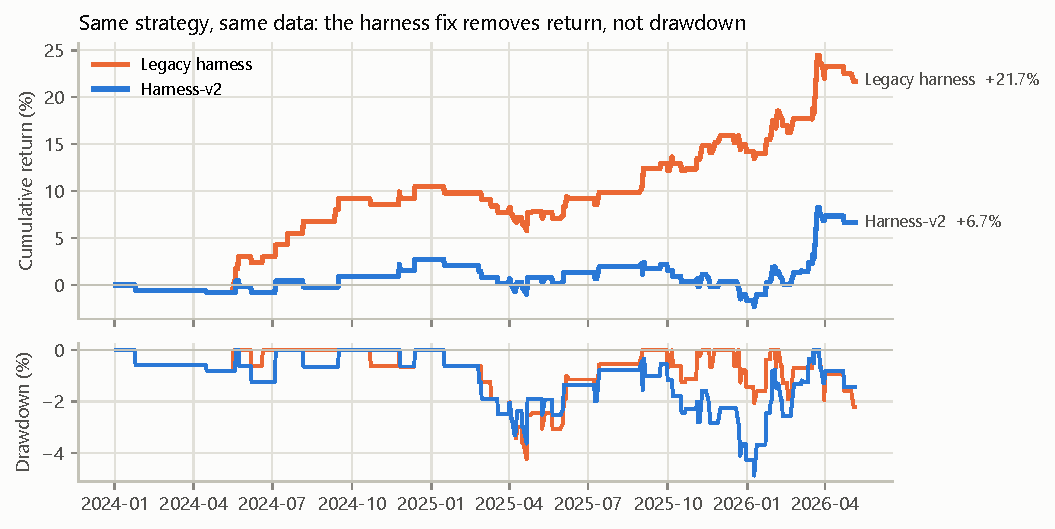
\includegraphics[width=\linewidth]{figures/F2_g0_equity.pdf}
\caption{\csuse{cap-F2}}
\label{fig:F2}
\end{figure}

\subsection{Order-block strategy: a re-measurement inside the in-sample period}
\label{sec:res-remeasure}

Earlier project documents reported that the strategy's best-looking refinement---signals with at
least two ``timing'' flags---``collapsed out of sample''. That comparison is reported here with
corrected units and an accurate description. It is \emph{not} an out-of-sample test.
\begin{itemize}
\item The in-sample figures come from a full-period run (December 2024 to May 2026). The
comparison figures come from five short windows between February 2025 and April 2026, run later
on newer code with transaction costs off. All five windows lie inside the in-sample period. % [C36, C37, C65]
\item The refinement was chosen after the in-sample results had been seen.
\item Both runs predate the corrected harness, so both contain the lookahead. % [C38]
\end{itemize}

Measured per signal on both sides, the refinement moves from $t=+3.045$ ($n=228$) in-sample to
$t=+0.06$ ($n=37$) in the re-run windows; the whole cohort moves from $+2.18$ ($n=514$) to $+0.63$
($n=43$). % [C30, C31, C34]
The re-measurement has little power. If the in-sample per-signal Sharpe ratio
($3.045/\sqrt{228}\approx0.20$) were the true value, the expected $t$ at $n=37$ would be about
$0.20\sqrt{37}\approx1.2$, and the observed $+0.06$ lies about one standard error below that,
inside the band of outcomes consistent with a real effect (Figure~\ref{fig:F7}). On its own, this
comparison is weak evidence against the refinement.

For completeness, an anchored walk-forward run on the legacy harness (minimum score 75, per-leg
statistics) gave positive results in all three six-month test windows, with $t$ of $+1.62$,
$+1.02$ and $+2.91$; none reached 3.0. % [C39, C41]
A later cost-aware walk-forward run reached $t=2.5$ in none of the three windows. % [C40]
Both runs contain the lookahead.

\begin{figure}[htbp]
\centering
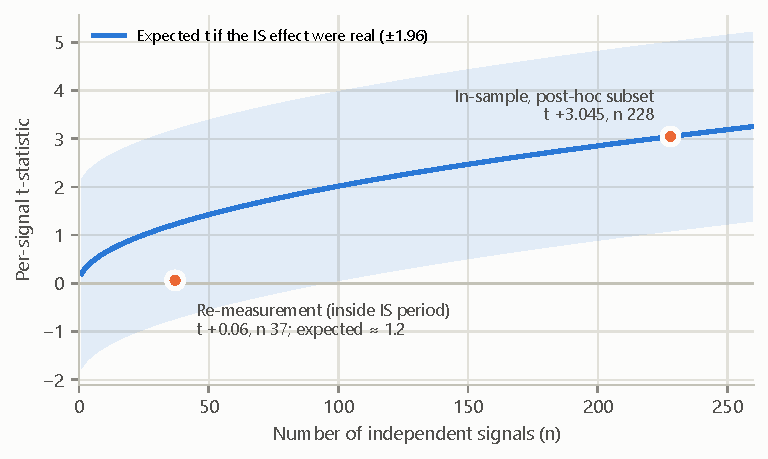
\includegraphics[width=0.78\linewidth]{figures/F7_power_band.pdf}
\caption{\csuse{cap-F7}}
\label{fig:F7}
\end{figure}

\subsection{Supply/demand-zone strategy: development stage}
\label{sec:res-zone}

The frozen specification (trial~1) and three variants were run on the DEV partition
(Table~\ref{tab:zone}, Figure~\ref{fig:F4}). Trials~2--4 were selected after trial~1 under the
specification's DEV-tuning permission; all four remained negative. They varied the two parameters
that most directly control zone quality: the impulse threshold and the maximum zone age.

\begin{table}[htbp]
\centering\small
\caption{Zone strategy on the DEV partition (2024), per signal, costs on, 0.5\% risk. Rows 1--4
of the trial ledger.}
\label{tab:zone}
\begin{tabular}{@{}llrrrrrr@{}}
\toprule
Trial & Variant & $n$ & PF & $E[\R]$ & $t$ (profit) & $t$ ($\R$) & Max DD (\%) \\
\midrule
1 & frozen v1.0 & 406 & 0.745 & $-0.143$ & $-2.79$ & $-2.92$ & 29.8 \\ % [C21]
2 & impulse $2.0\times$ATR & 240 & 0.772 & $-0.126$ & $-1.90$ & $-1.94$ & 17.4 \\ % [C22]
3 & maximum age 24 bars & 334 & 0.775 & $-0.124$ & $-2.21$ & $-2.28$ & 22.6 \\ % [C23]
4 & both & 187 & 0.744 & $-0.141$ & $-1.92$ & $-1.92$ & 13.4 \\ % [C24]
\bottomrule
\end{tabular}
\end{table}

\begin{figure}[htbp]
\centering
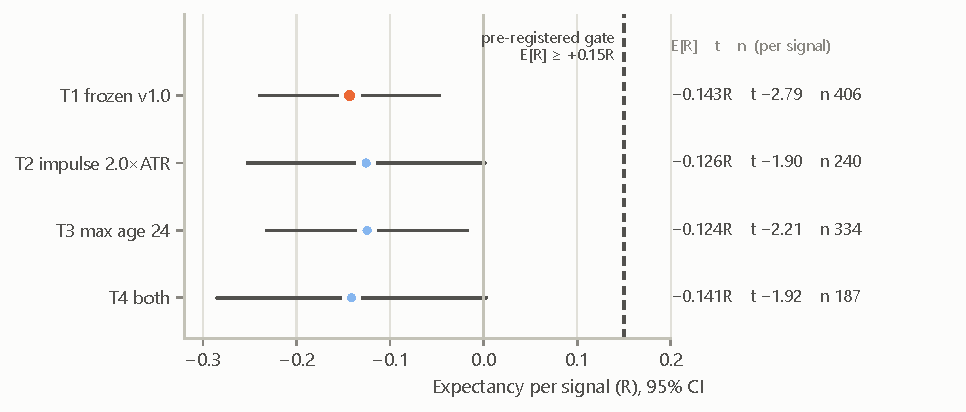
\includegraphics[width=0.92\linewidth]{figures/F4_zone_dev.pdf}
\caption{\csuse{cap-F4}}
\label{fig:F4}
\end{figure}

The frozen specification is far from its gate: $t=-2.79$ against $+2.5$, expectancy
$-0.143\R$ against $+0.15\R$, and maximum drawdown 29.8\% against 6\%. % [C19, C21]
Its 95\% interval for expectancy excludes zero; the intervals for trials~2 and~4 just reach zero. % [C75]
Three diagnostics describe the loss:
\begin{itemize}
\item \textbf{Direction.} Both sides lose: 208 sell signals and 198 buy signals both have negative
mean profit, in a year in which gold rose strongly. The loss is not exposure to the trend. % [C25]
\item \textbf{Costs.} Commission and swap account for about $-0.018\R$ of the $-0.143\R$;
without them expectancy would still be about $-0.125\R$. % [C27]
\item \textbf{Quality.} Tightening the two quality parameters cut the number of signals from 406
to 187 but left expectancy between $-0.14\R$ and $-0.12\R$. If touches of stronger zones carried
an edge, stricter filters would concentrate it; they did not. % [C21–C24]
\end{itemize}
Of 5,912 H1 bars, 1,595 produced swings, 656 produced active zones, 508 zones were touched and 406
signals were traded (Figure~\ref{fig:F5}). % [C28]

Under the specification's failure rule the study stopped at this stage. The EVAL and FRESH
partitions were not used, and the ledger holds four rows. % [C20, C29]

\begin{figure}[htbp]
\centering
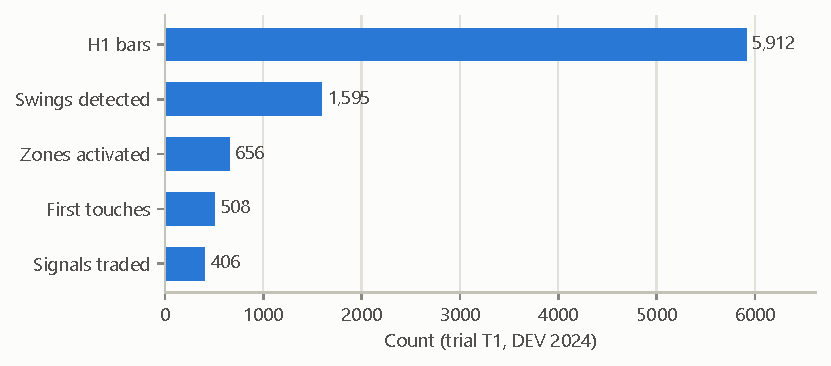
\includegraphics[width=0.7\linewidth]{figures/F5_zone_funnel.pdf}
\caption{\csuse{cap-F5}}
\label{fig:F5}
\end{figure}

\subsection{Register of documented ideas}
\label{sec:res-register}

Table~\ref{tab:ideas} lists every idea for which a primary artifact or a dated contemporaneous
record exists (Figure~\ref{fig:F6}). Project notes mention a larger total of about nineteen ideas;
that total could not be reconstructed from primary artifacts, so only the fifteen documented
ideas are listed. Labels are defined as follows.
\textsc{Falsified}: a pre-registered gate failed and the estimate is significantly on the wrong
side, or the gate failure is unambiguous.
\textsc{Not supported}: tested, but the evidence for edge does not reach the bar.
\textsc{Inconclusive}: measured, but the result cannot discriminate.
\textsc{Not tested}: tooling exists but no result does.
Ideas marked ``recorded, not re-run'' rest on a dated record whose generating script exists but
whose output was not saved; they were not re-run for this report.

{\small
\begin{longtable}{@{}p{0.45cm}>{\raggedright\arraybackslash}p{3.6cm}>{\raggedright\arraybackslash}p{6.15cm}>{\raggedright\arraybackslash}p{3.0cm}@{}}
\caption{Register of the fifteen documented ideas. $\dagger$ = recorded, not re-run.}\label{tab:ideas}\\
\toprule
\# & Idea & Key result & Label \\
\midrule
\endfirsthead
\toprule
\# & Idea & Key result & Label \\
\midrule
\endhead
1 & Order-block confluence (frozen) & Corrected harness: per-signal $t=+0.92$, $n=77$ & \textsc{Not supported} \\ % [C07, C08]
2 & Order-block $\geq$2-flag refinement & $t=+3.045$ ($n=228$, post hoc) $\rightarrow$ $+0.06$ ($n=37$), within-sample re-measurement & \textsc{Not supported} \\ % [C31, C34]
3 & Supply/demand zone v1.0 & DEV: $t=-2.79$, $E[\R]=-0.143$, $n=406$ & \textsc{Falsified} \\ % [C21]
4 & Pending-limit execution & Gate failed: limit PF 1.599 below market PF 1.718 & \textsc{Not supported} \\ % [C44]
5 & Hourly entry with limit orders$\dagger$ & $t=1.98$ on 12 fills, below 2.5 & \textsc{Not supported} \\ % [C45]
6 & Hidden-Markov regime filter & Met its own pre-registered Sharpe criterion; 0 of 3 windows reach $t=2.5$; legacy harness & \textsc{Inconclusive} \\ % [C43]
7 & Language-model trade filter$\dagger$ & 11 approved trades, $p=1.00$ & \textsc{Inconclusive} \\ % [C49]
8 & Machine learning on M15 price features$\dagger$ & AUC 0.491--0.503; positive control 0.693 & \textsc{Not supported} \\ % [C46]
9 & Volatility risk premium$\dagger$ & Implied exceeded realised volatility by 4.05 points on 85.3\% of days; worst month $-309\%$ & \textsc{Not supported}\textsuperscript{a} \\ % [C47]
10 & Crypto order-flow imbalance$\dagger$ & Net $-2.80$ to $-4.05$ basis points per trade & \textsc{Not supported} \\ % [C48]
11 & Cointegration pairs (16) & 0 of 16 pairs pass FDR, frozen-$\beta$ and half-life tests & \textsc{Falsified} \\ % [C50]
12 & Crypto cross-sectional momentum$\dagger$ & Deflated Sharpe 0.21 at the honest trial count & \textsc{Falsified} \\ % [C51]
13 & Portfolio time-series momentum (41 assets) & Phase 1 passed (Deflated Sharpe 0.982, $N=86$); no significant alpha over a managed-futures ETF ($p=0.068$) & \textsc{Not supported}\textsuperscript{b} \\ % [C52, C53]
14 & Prediction-market basket arbitrage & Data snapshot only; no verdict & \textsc{Not tested} \\ % [C54]
15 & Grading third-party posted zone calls & Grader built and tested; never given data & \textsc{Not tested} \\ % [C55]
\bottomrule
\multicolumn{4}{@{}p{14cm}@{}}{\footnotesize \textsuperscript{a}The premium was present, but its
tail risk is incompatible with a 10\% drawdown limit. \textsuperscript{b}The premium was present,
but it is not significant beyond a publicly traded managed-futures fund (ex-crypto $p=0.156$).}\\
\end{longtable}
}

\begin{figure}[htbp]
\centering
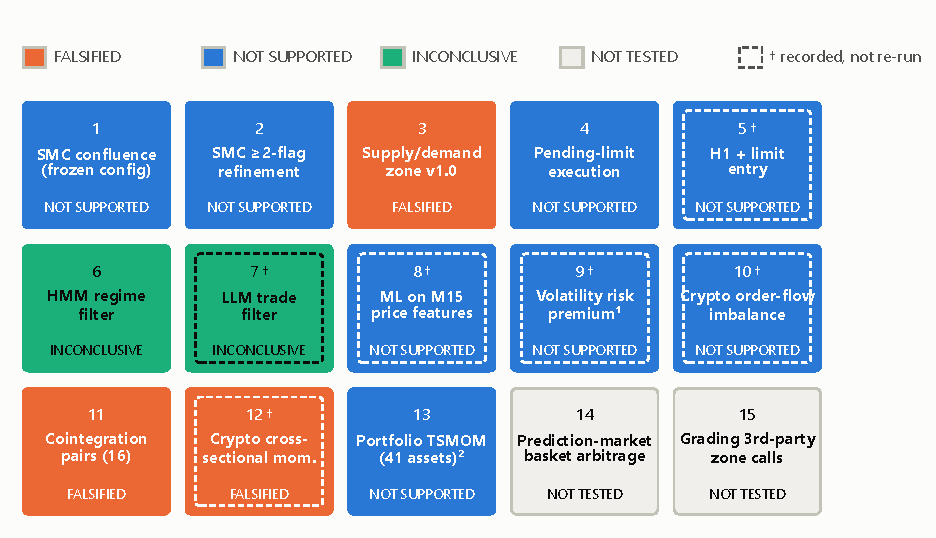
\includegraphics[width=0.9\linewidth]{figures/F6_idea_register.pdf}
\caption{\csuse{cap-F6}}
\label{fig:F6}
\end{figure}

% ════════════════════════════════════════════════════════════════════════════
\FloatBarrier
\section{Discussion}
\label{sec:discussion}

\subsection{What the evidence shows}
Under a causal harness and per-signal inference, neither price-structure rule family shows a
measurable per-signal edge on this instrument and period. The two results differ in kind. The
order-block result is a null: a positive point estimate whose interval includes zero. The zone
result is significantly negative under its frozen specification, symmetric between long and
short, not explained by costs, and insensitive to the quality filters that the premise says
should matter.

\subsection{What the evidence does not show}
It does not show that these rules cannot work elsewhere: one instrument, one data vendor and one
period were examined, and the zone strategy was evaluated on its development partition only. It
does not show that the order-block strategy has zero edge, only that the evidence for an edge is
far below any reasonable bar. And the within-sample re-measurement of
Section~\ref{sec:res-remeasure} is weak evidence in either direction.

\subsection{Harness defects inflate the mean, not the variance}
In the calibration, expectancy fell by 62\% while the maximum drawdown stayed near 5\%
(Table~\ref{tab:g0}). The lookahead improved the \emph{selection and outcome} of trades---the
numerator of the $t$-statistic---while leaving the dispersion of outcomes largely unchanged.
Large in-sample significance alongside ordinary drawdowns is a pattern worth checking for.

\subsection{The lookahead cannot explain the in-sample to re-measurement gap}
Both sides of the comparison in Section~\ref{sec:res-remeasure} ran on the legacy harness, so the
lookahead affected both and cannot account for the difference between them. % [C38]
The more economical explanation is selection: the refinement was chosen after the in-sample
results were seen, from a score that in practice varies along a single dimension, since five of
its six flags are almost always on or almost always off among traded signals (recorded, not
re-run). % [C42]
The re-measurement is too small to distinguish selection from a real but noisy effect; the
corrected-harness calibration is what carries the conclusion.

\subsection{Relation to the order-clustering literature}
The order-data evidence of \citet{osler2003currency,osler2005stoploss} concerns levels at which
orders are documented to sit. Retail-drawn order blocks and zones are not shown here to coincide
with such levels. The zone test measured the payoff to entering on a touch directly and found it
negative; this is what one would expect if the drawn levels are not where offsetting orders
actually wait.

\subsection{Corrections to earlier project documents}
\label{sec:corrections}
Three statements in earlier project documents are corrected here. The original documents are
preserved unchanged; corrections are recorded as new dated notes.
\begin{enumerate}
\item \textbf{Unit mismatch.} The statement ``in-sample $t=+3.05$, out-of-sample $t=+0.09$''
compared a per-signal in-sample statistic with a per-leg statistic from the comparison windows.
Per signal on both sides, the figures are $+3.045$ and $+0.06$. % [C35]
\item \textbf{Mislabelled out-of-sample test.} The comparison windows lie inside the in-sample
period, were run on newer code with costs off, and are short ad-hoc windows rather than
walk-forward folds. The comparison is a within-sample re-measurement. % [C36, C37]
\item \textbf{Configuration label.} A walk-forward note gave the minimum score as 65; the
artifact shows that no trade below 75 was taken, consistent with the configuration change dated
three days before the run. % [C41]
\end{enumerate}

% ════════════════════════════════════════════════════════════════════════════
\section{Limitations}
\label{sec:limits}

\begin{itemize}
\item \textbf{One instrument, one data source.} Only XAUUSD was studied, using Dukascopy BID
quotes. A broker's own feed differs in spreads and timestamps. % [C63]
\item \textbf{Bar-based fill simulation.} Exits are resolved from bar highs and lows. When a
stop-loss and a take-profit are both touched inside one bar, the stop is assumed to have been hit
first; a bar that opens beyond either level fills at the open. The true intra-bar order is
unknown. % [C66]
\item \textbf{Live and backtest information sets differ.} The live system's data feed includes
the current, still-forming bar and the strategy reads its latest values, whereas the corrected
backtest uses only closed bars. The backtest therefore does not reproduce the live decision rule
exactly, and the direction and size of the effect on results have not been measured. % [C67]
\item \textbf{The trial ledger started late.} The ledger began with the zone study. Earlier
order-block work tried many configurations that were not recorded, so any Deflated Sharpe Ratio
computed for that work with a small $N$ is optimistic.
\item \textbf{Controls and live costs not yet measured.} No null control has been run on the
corrected harness, live execution costs and slippage have not been measured against the backtest
assumption, and the forward demonstration test has about 0 of its required 30 trades. % [C56]
\item \textbf{Records not re-run.} Six ideas in Table~\ref{tab:ideas} rest on dated records
whose outputs were not saved.
\item \textbf{Self-reported timestamps.} The pre-registration timeline relies on version-control
commit times recorded by the author's machine, which are not externally notarised. % [C68]
\item \textbf{AI-assisted development.} The software and analyses were developed with an AI
coding assistant; see the disclosure in Appendix~\ref{app:disclosure}.
\end{itemize}

% ════════════════════════════════════════════════════════════════════════════
\section{Conclusion}

On XAUUSD 5-minute data, two retail price-structure rule families were examined under a causal
backtest with per-signal inference. The order-block strategy's apparent edge was largely a
product of two harness defects: once they were corrected on identical data and code, its
per-signal $t$-statistic fell from $+2.45$ to $+0.92$. A supply/demand-zone strategy, specified
and committed before its first backtest result, failed its pre-registered gate at the development stage with a
significantly negative expectancy, and the evaluation data were left unused. Neither result
supports trading these rules. The durable outputs of the project are the validation tooling---close-time
slicing with a mandatory test, per-signal statistics, an append-only trial ledger---and the
practice of measuring an idea before believing it.

% ════════════════════════════════════════════════════════════════════════════
\FloatBarrier
\bibliographystyle{plainnat}
\bibliography{references_verified}

\appendix
\section{Reproducibility}
\label{app:repro}

\subsection{File map}
The public evidence bundle mirrors the project layout. The main groups:
\begin{itemize}[before=\raggedright]
\item \texttt{report\_calib\_v1\_full.json}, \texttt{report\_calib\_v2\_full.json}: calibration
runs (Table~\ref{tab:g0}); \texttt{report\_costs\_065.json}: the recorded legacy artifact.
\item \texttt{report\_zone\_dev\_t1.json}--\texttt{t4.json}, \texttt{trials.csv},
\texttt{specs/phase1\_zone\_spec\_v1.md}, \texttt{reports/phase2/DEV\_report.md}: the zone study.
\item \texttt{report\_full.json}, \texttt{report\_w1.json}--\texttt{w5.json}: the within-sample
re-measurement; \texttt{wfv\_*.json}: walk-forward runs.
\item \texttt{backtest/}, \texttt{quant/}, \texttt{core/}, \texttt{tools/}, \texttt{tests/}: the
code that produced the results and the code cited in the limitations; \texttt{research/}: records for ideas 11--14 (the cointegration result is vendored into
the repository, so the build reads no file outside it).
\item \texttt{paper/claims.csv}: every number in this report, with source file and locator.
\end{itemize}

\subsection{Re-running the checks}
With the project's Python environment:
\begin{itemize}[before=\raggedright]
\item \texttt{python -m tests.test\_no\_lookahead} (1,000-step causality test);
\texttt{python -m tests.test\_per\_signal\_metrics}; \texttt{python -m tests.test\_zone\_engine};
\texttt{python -m tests.test\_zone\_runner}.
\item \texttt{python backtest/\_flag\_analysis.py report\_w1.json \ldots{} report\_w5.json}
(Section~\ref{sec:res-remeasure}, per-leg and per-signal).
\item \texttt{python -m backtest.zone\_cli} with the parameters in \texttt{trials.csv} (zone
trials; each run appends a ledger row).
\item \texttt{python paper/figures/make\_figures.py --root .} (all figures and their captions;
requirements in \texttt{paper/requirements-figures.txt}).
\item \texttt{data/\_fetch\_dukascopy\_2024.py} (price data; compare against the hash below).
\end{itemize}
In the public repository, \texttt{tests.test\_no\_lookahead} and \texttt{tests.test\_zone\_runner}
need the price data or the live system's configuration module, neither of which is published, and
are reported as skipped.

\subsection{Hashes of the public files}
The table lists the SHA-256 (first 16 hexadecimal digits; full values in
\texttt{SHA256SUMS.txt}) of every file in the public evidence bundle. Six files were redacted;
\textbf{the only change made by redaction was replacing the original project folder name with the
token \texttt{project}}. Four files are not published and are listed with the hash of the
original: the price data (redistribution terms not verified), a fault-injection log and one
dated note that contain a demonstration-account identifier, and the project status file, which
names the broker and the account balance. Their full hashes are in
\texttt{EXCLUDED.SHA256SUMS.txt}, so that a reader who regenerates the price data can verify it.
The audit script reports any check that needs an unpublished file as \emph{skipped}, never as
passed, when the file is absent.

{\scriptsize
\begin{longtable}{@{}>{\raggedright\arraybackslash}p{8.6cm}p{2.7cm}>{\raggedright\arraybackslash}p{3.4cm}@{}}
\toprule
File & SHA-256 (prefix) & Status \\
\midrule
\endhead
\texttt{data/\allowbreak{}xauusd\_m5\_full.csv} & \texttt{86271f9b6fb4e3fd} & not published (hash of original) \\
\texttt{data/\allowbreak{}\_fetch\_dukascopy\_2024.py} & \texttt{d4002cefd405685c} & verbatim \\
\texttt{trials.csv} & \texttt{8334fec3d4328530} & verbatim \\
\texttt{report\_costs\_065.json} & \texttt{0222ae8b91756bac} & verbatim \\
\texttt{bt\_costs\_065.log} & \texttt{db8526f5c1faaaaf} & verbatim \\
\texttt{report\_calib\_v1\_full.json} & \texttt{611cf0bbc7003970} & verbatim \\
\texttt{report\_calib\_v2\_full.json} & \texttt{c71ed4c181c1f610} & verbatim \\
\texttt{bt\_calib\_v1.err.log} & \texttt{fff56ea2769ced38} & redacted (2 replacements) \\
\texttt{bt\_calib\_v2.err.log} & \texttt{966a9abc0459bf5d} & redacted (30 replacements) \\
\texttt{reports/\allowbreak{}phase0/\allowbreak{}G0\_report.md} & \texttt{4af0b3a88a5079a3} & redacted (1 replacement) \\
\texttt{reports/\allowbreak{}phase0/\allowbreak{}diff\_0.1\_lookahead\_fix.patch} & \texttt{b4cf3193f6a59803} & redacted (6 replacements) \\
\texttt{reports/\allowbreak{}phase0/\allowbreak{}diff\_0.2\_per\_signal\_stats.md} & \texttt{0617b21a7b3d05d1} & verbatim \\
\texttt{reports/\allowbreak{}phase0/\allowbreak{}calib\_json\_sha256.txt} & \texttt{8978645fc696cf2f} & verbatim \\
\texttt{reports/\allowbreak{}phase0/\allowbreak{}report\_calib\_v1\_smoke.json} & \texttt{9416ed1809dbe99a} & verbatim \\
\texttt{reports/\allowbreak{}phase0/\allowbreak{}report\_calib\_v2\_smoke.json} & \texttt{9416ed1809dbe99a} & verbatim \\
\texttt{reports/\allowbreak{}phase0/\allowbreak{}bt\_calib\_v1\_attempt1\_crash.log} & \texttt{da988159c0276538} & redacted (11 replacements) \\
\texttt{specs/\allowbreak{}phase1\_zone\_spec\_v1.md} & \texttt{03ddb7b216a925c0} & redacted (1 replacement) \\
\texttt{reports/\allowbreak{}phase2/\allowbreak{}DEV\_report.md} & \texttt{f2a16fe6b48399b3} & verbatim \\
\texttt{report\_zone\_dev\_t1.json} & \texttt{8e78f735b0f4b135} & verbatim \\
\texttt{report\_zone\_dev\_t2.json} & \texttt{680cfa7bc39d4ac3} & verbatim \\
\texttt{report\_zone\_dev\_t3.json} & \texttt{cabb08e7febc8bc5} & verbatim \\
\texttt{report\_zone\_dev\_t4.json} & \texttt{3b6de201b05e0ac0} & verbatim \\
\texttt{report\_full.json} & \texttt{a7fedee66dc7badc} & verbatim \\
\texttt{report\_w1.json} & \texttt{8c76ed83a99772f3} & verbatim \\
\texttt{report\_w2.json} & \texttt{476833c1c1aa009c} & verbatim \\
\texttt{report\_w3.json} & \texttt{cd33449fc8eec236} & verbatim \\
\texttt{report\_w4.json} & \texttt{a849526720e1a6c8} & verbatim \\
\texttt{report\_w5.json} & \texttt{ecfc8198f9d91cf1} & verbatim \\
\texttt{report\_prefix.json} & \texttt{8898ed82d66324b9} & verbatim \\
\texttt{report\_postfix.json} & \texttt{8898ed82d66324b9} & verbatim \\
\texttt{wfv\_report.json} & \texttt{a3dc15dfa9f50c0b} & verbatim \\
\texttt{wfv\_baseline\_75.json} & \texttt{f07a8b665eda1e23} & verbatim \\
\texttt{wfv\_hmm\_report.json} & \texttt{d7879cef6fda776b} & verbatim \\
\texttt{report\_limit\_vs\_market.json} & \texttt{33d6801c11b06c4a} & verbatim \\
\texttt{tools/\allowbreak{}\_configB\_oos.json} & \texttt{36a77c746a8dd01d} & verbatim \\
\texttt{tools/\allowbreak{}\_configB\_exp4.json} & \texttt{ec0035833e3f6bd9} & verbatim \\
\texttt{research/\allowbreak{}tsmom\_portfolio/\allowbreak{}RESULTS.md} & \texttt{28b419edd88bf6f6} & verbatim \\
\texttt{research/\allowbreak{}tsmom\_portfolio/\allowbreak{}run\_log.txt} & \texttt{c9d2f84955210870} & verbatim \\
\texttt{research/\allowbreak{}tsmom\_portfolio/\allowbreak{}PHASE2\_SUMMARY.md} & \texttt{87320cdf3e460fa9} & verbatim \\
\texttt{research/\allowbreak{}tsmom\_portfolio/\allowbreak{}phase2\_run\_log.txt} & \texttt{37fa31cd3c22991d} & verbatim \\
\texttt{research/\allowbreak{}xs\_crypto\_momentum/\allowbreak{}RESULTS.md} & \texttt{48f4a492098dcd7a} & verbatim \\
\texttt{research/\allowbreak{}polymarket\_arb/\allowbreak{}snapshot\_existence.json} & \texttt{e1ce759409f3f4af} & verbatim \\
\texttt{.claude/\allowbreak{}skills/\allowbreak{}quant-\allowbreak{}trading/\allowbreak{}lessons/\allowbreak{}2026-\allowbreak{}05-\allowbreak{}29-\allowbreak{}walk-\allowbreak{}forward-\allowbreak{}results.md} & \texttt{155831b287b99313} & verbatim \\
\texttt{.claude/\allowbreak{}skills/\allowbreak{}quant-\allowbreak{}trading/\allowbreak{}lessons/\allowbreak{}2026-\allowbreak{}05-\allowbreak{}29-\allowbreak{}pending-\allowbreak{}limit-\allowbreak{}order-\allowbreak{}system.md} & \texttt{fc59a457d8ca53a4} & verbatim \\
\texttt{.claude/\allowbreak{}skills/\allowbreak{}quant-\allowbreak{}trading/\allowbreak{}lessons/\allowbreak{}2026-\allowbreak{}05-\allowbreak{}31-\allowbreak{}hmm-\allowbreak{}regime-\allowbreak{}detection.md} & \texttt{52ec0f7a8d5c3381} & verbatim \\
\texttt{.claude/\allowbreak{}skills/\allowbreak{}quant-\allowbreak{}trading/\allowbreak{}lessons/\allowbreak{}2026-\allowbreak{}06-\allowbreak{}03-\allowbreak{}phase0-\allowbreak{}execution-\allowbreak{}hardening.md} & \texttt{873ea28115830546} & verbatim \\
\texttt{.claude/\allowbreak{}skills/\allowbreak{}quant-\allowbreak{}trading/\allowbreak{}lessons/\allowbreak{}2026-\allowbreak{}06-\allowbreak{}05-\allowbreak{}llm-\allowbreak{}htf-\allowbreak{}demotion.md} & \texttt{6b8b50bf6cf8be20} & not published (hash of original) \\
\texttt{.claude/\allowbreak{}skills/\allowbreak{}quant-\allowbreak{}trading/\allowbreak{}lessons/\allowbreak{}2026-\allowbreak{}06-\allowbreak{}10-\allowbreak{}backtest-\allowbreak{}on2-\allowbreak{}and-\allowbreak{}desync.md} & \texttt{1b7084b22b787ae6} & verbatim \\
\texttt{.claude/\allowbreak{}skills/\allowbreak{}quant-\allowbreak{}trading/\allowbreak{}lessons/\allowbreak{}2026-\allowbreak{}06-\allowbreak{}13-\allowbreak{}h1-\allowbreak{}limit-\allowbreak{}phase1.md} & \texttt{bc03bf3643d63957} & verbatim \\
\texttt{.claude/\allowbreak{}skills/\allowbreak{}quant-\allowbreak{}trading/\allowbreak{}lessons/\allowbreak{}2026-\allowbreak{}06-\allowbreak{}13-\allowbreak{}signal-\allowbreak{}rootcause-\allowbreak{}smc-\allowbreak{}degenerate.md} & \texttt{65e4c95cdd797ec3} & verbatim \\
\texttt{.claude/\allowbreak{}skills/\allowbreak{}quant-\allowbreak{}trading/\allowbreak{}lessons/\allowbreak{}2026-\allowbreak{}06-\allowbreak{}16-\allowbreak{}strategy-\allowbreak{}exhaustion-\allowbreak{}and-\allowbreak{}pivot-\allowbreak{}research.md} & \texttt{2481556818075d37} & verbatim \\
\texttt{.claude/\allowbreak{}skills/\allowbreak{}quant-\allowbreak{}trading/\allowbreak{}lessons/\allowbreak{}2026-\allowbreak{}07-\allowbreak{}05-\allowbreak{}harness-\allowbreak{}v2-\allowbreak{}calibration-\allowbreak{}anchor.md} & \texttt{41aca7ef42c37f5f} & verbatim \\
\texttt{.claude/\allowbreak{}skills/\allowbreak{}quant-\allowbreak{}trading/\allowbreak{}lessons/\allowbreak{}2026-\allowbreak{}07-\allowbreak{}15-\allowbreak{}zone-\allowbreak{}strategy-\allowbreak{}verdict.md} & \texttt{2efcdce0b6ddd27d} & verbatim \\
\texttt{backtest/\allowbreak{}data\_loader.py} & \texttt{fef8ce1a35854661} & verbatim \\
\texttt{backtest/\allowbreak{}metrics.py} & \texttt{6b2f6b52f322eb84} & verbatim \\
\texttt{backtest/\allowbreak{}virtual\_broker.py} & \texttt{2f2805c6151aa4bc} & verbatim \\
\texttt{backtest/\allowbreak{}walk\_forward.py} & \texttt{50dacc6d35cb5e6d} & verbatim \\
\texttt{backtest/\allowbreak{}zone\_runner.py} & \texttt{22bbad455029f3e9} & verbatim \\
\texttt{backtest/\allowbreak{}zone\_cli.py} & \texttt{4823affa4b7ac440} & verbatim \\
\texttt{backtest/\allowbreak{}\_flag\_analysis.py} & \texttt{8f2b1abf339ee758} & verbatim \\
\texttt{quant/\allowbreak{}zone\_engine.py} & \texttt{12581834c16d2c50} & verbatim \\
\texttt{tools/\allowbreak{}trials\_ledger.py} & \texttt{c004320b77db4892} & verbatim \\
\texttt{tools/\allowbreak{}track\_a\_grader.py} & \texttt{417b6723191a534f} & verbatim \\
\texttt{agents/\allowbreak{}risk\_manager.py} & \texttt{1dfa09df59084abe} & verbatim \\
\texttt{execution/\allowbreak{}order\_executor.py} & \texttt{f3fdfe9f9b680891} & verbatim \\
\texttt{memory/\allowbreak{}trade\_logger.py} & \texttt{1688bb607d715397} & verbatim \\
\texttt{core/\allowbreak{}event\_bus.py} & \texttt{9d08645d45403b69} & verbatim \\
\texttt{main.py} & \texttt{a01eb656a6ec7efd} & verbatim \\
\texttt{tests/\allowbreak{}test\_no\_lookahead.py} & \texttt{875305ae0c521f07} & verbatim \\
\texttt{tests/\allowbreak{}test\_per\_signal\_metrics.py} & \texttt{a94e3f915c1fdf2c} & verbatim \\
\texttt{tests/\allowbreak{}test\_zone\_engine.py} & \texttt{98f267fdfb706b17} & verbatim \\
\texttt{tests/\allowbreak{}test\_zone\_runner.py} & \texttt{a63e42e396c270f7} & verbatim \\
\texttt{tests/\allowbreak{}test\_track\_a\_grader.py} & \texttt{158a0f665939b5e9} & verbatim \\
\texttt{logs/\allowbreak{}chaos.log} & \texttt{8d1ab4b425c0621a} & not published (hash of original) \\
\texttt{.claude/\allowbreak{}skills/\allowbreak{}quant-\allowbreak{}trading/\allowbreak{}lessons/\allowbreak{}2026-\allowbreak{}11-\allowbreak{}01-\allowbreak{}wfv-\allowbreak{}min-\allowbreak{}score-\allowbreak{}correction.md} & \texttt{e5a2397a482e9eb2} & verbatim \\
\texttt{research/\allowbreak{}cointegration/\allowbreak{}phase1\_results.json} & \texttt{eef742e8865bd09f} & verbatim \\
\texttt{core/\allowbreak{}data\_stream.py} & \texttt{64d2a88d442d29dc} & verbatim \\
\texttt{quant/\allowbreak{}smc\_engine.py} & \texttt{cc7819214cfa492d} & verbatim \\
\texttt{PROJECT\_STATUS.md} & \texttt{889e5c57dc7004eb} & not published (hash of original) \\
\bottomrule
\end{longtable}
}


\section{Disclosure}
\label{app:disclosure}
The author is a high-school student. The trading system, the backtests and this report were
developed with an AI coding assistant, under the author's design and review. The report has not
been peer-reviewed. No real capital was traded in any of the studies reported here.

\end{document}
